\documentclass[11pt]{article}

% Document settings, taken from Introduction to Algorithms (Dinitz).
\usepackage{epsfig}
\usepackage{amsfonts}
\usepackage{amssymb}
\usepackage{amstext}
\usepackage{amsmath}
\usepackage{xspace}
\usepackage{hyperref}
\usepackage{fullpage}
\usepackage{enumitem}                     
\usepackage{titlesec}
\usepackage{amsthm}
\usepackage{natbib}

\hypersetup{
    colorlinks=true,
    linkcolor=blue,
    filecolor=magenta,      
    urlcolor=cyan,
}

\titleformat*{\section}{\bfseries}
\titleformat*{\subsection}{\bfseries}
\titleformat*{\subsubsection}{\bfseries}
\titleformat*{\paragraph}{\bfseries}
\titleformat*{\subparagraph}{\bfseries}

\newcommand{\R}{\ensuremath{\mathbb R}}
\newcommand{\C}{\ensuremath{\mathbb C}}
\newcommand{\N}{\ensuremath{\mathbb N}}
\newcommand{\F}{\ensuremath{\mathbb F}}
\newcommand{\K}{\ensuremath{\mathbb K}}
\newcommand{\Z}{\ensuremath{\mathbb Z}}
\newcommand{\B}{\ensuremath{\mathcal B}}
\renewcommand{\H}{\ensuremath{\mathcal H}}
\newcommand{\EV}{\ensuremath{\mathbb E}}
\newcommand{\Var}{\text{Var}}
\newcommand{\Cov}{\text{Cov}}
\newcommand{\e}{\epsilon}
\newcommand{\E}{\exists}
\newcommand{\sse}{\subseteq}
\newcommand{\union}{\cup}
\newcommand{\ra}{\rightarrow}
\newcommand{\ceil}[1]{\ensuremath{\left\lceil#1\right\rceil}}
\newcommand{\floor}[1]{\ensuremath{\left\lfloor#1\right\rfloor}}
\newcommand{\ip}[2]{\left\langle #1, #2\right\rangle}
\DeclareMathOperator*{\argmax}{arg\,max\ }
\DeclareMathOperator*{\argmin}{arg\,min\ }

\theoremstyle{plain}
\newtheorem{thm}{Theorem}[section]
\newtheorem{lem}{Lemma}[section]
\newtheorem{prop}{Proposition}[section]
\newtheorem{coro}{Corollary}[section]
\newtheorem{obs}{Observation}[section]

\theoremstyle{definition}
\newtheorem{defi}{Definition}[section]

\theoremstyle{remark}
\newtheorem{exm}{Example}[section]
\newtheorem{exc}{Exercise}[section]
\newtheorem{rem}{Remark}[section]
\newtheorem{question}{Question}
\newtheorem{answer}{Answer}

\setenumerate[0]{label=(\alph*)}


%%%%%%%%%%%%%%%%%%%%%%%%%%%%%%%%%%%%%%%%%%%%%%%%%%%%%%%%%%%%%%%%%%%%%%%%%%%
%%%%%%%%%%%%%%%%%%%%%%%%%% Document begins here %%%%%%%%%%%%%%%%%%%%%%%%%%%
%%%%%%%%%%%%%%%%%%%%%%%%%%%%%%%%%%%%%%%%%%%%%%%%%%%%%%%%%%%%%%%%%%%%%%%%%%%


\begin{document}

% EDIT THE FOLLOWING PARAMETERS FOR EACH ASSIGNMENT.

% NAME and COURSE TITLE + SECTION NUMBER
\noindent {\large {\bf Mathematical Thinking and Proof-Writing for Engineers}} \hfill {\bf Intersession 2020}

% PROFESSOR and HOMEWORK NUMBER
\noindent {{\bf Instructor:} Ronak Mehta} \hfill 
{Class Notes}

\noindent \rule[0.1in]{\textwidth}{0.4pt}

% CONTENT

\section{January 6, 2020}

\paragraph{Prereading} \href{https://drive.google.com/drive/folders/1T_M-dvYE4leOSmpKt2eGYOvPRch_SDpK?usp=sharing}{Pages 1 - 11} of {\it Mathematics: A Discrete Introduction} by Edward Scheinerman.

\subsection{Introduction}
Welcome, and thanks for your interest! While mathematical theory is usually not the poster boy of engaging and topical intersession courses, I think we can change some minds with this particular class. The subject is fascinating, but notoriously difficult to teach. There are many balancing acts when it comes to mathematical education; those of memorization versus exploration, theory versus application, and lectures versus self-guided learning constitute most of the battle. In any case, I can make a strong argument for the utility of this course in your future endeavors, so I'll attempt to present it in a way that is best for you. To this end, I ask of you all a healthy amount of honest and constructive feedback throughout the course.

As a brief introduction, I recently graduated from the Master's program in Applied Mathematics and Statistics at Hopkins in May. Generally, I have focused my education around the mathematical foundations of data science - namely statistics, linear algebra, and optimization. I currently work in the \href{https://neurodata.io/}{lab of Dr. Joshua Vogelstein} in the Department of Biomedical Engineering, where I develop statistical procedures for neuroimaging data. I've also recently gone through a round of Ph.D. applications in data science, so hopefully you will hear some good news over the course of this class!

First, let us motivate this class, both in a general sense, and a way that applies to you directly. The most recent \href{https://hechingerreport.org/what-2018-pisa-international-rankings-tell-us-about-u-s-schools/}{Programme for International Student Assessment (PISA)} in 2018 ranked the U.S. at 36th out of 79 countries in mathematics. For decades, American math proficiency has compared abysmally to other developed nations, and since the 1980's the ``\href{https://en.wikipedia.org/wiki/Math_wars}{math wars}" debate pits rote memorization versus inquiry-based approaches to learning. I am personally unconvinced that such a dichotomy exists, given how many American debates typically present only two, fundamentally opposing options against one another. Moreover, these kinds of assessments come from a place of ``\href{http://neatoday.org/2019/12/03/2018-pisa-results/}{mental Olympics}" competitions for countries, as well as a measure of how prepared students are for a modern job market.  While this is a fine perspective, also consider the beauty and virtue that mathematics holds in and of itself. 

Paul Lockhart, in his book {\it A Mathematician's Lament}, compares current mathematics education to a dystopian version of teaching music.\\
\setlength{\leftskip}{1cm}

Since musicians are known to set down their ideas in the form of sheet music, these curious black dots and lines must constitute the ``language of music.” It is imperative that students become fluent in this language if they are to attain any degree of musical competence; indeed, it would be ludicrous to expect a child to sing a song or play an instrument without having a thorough grounding in music notation and theory. Playing and listening to music, let alone composing an original piece, are considered very advanced topics and are generally put off until college, and more often graduate school...

In the higher grades the pressure is really on. After all, the students must be prepared for the standardized tests and college admissions exams. Students must take courses in Scales and Modes, Meter, Harmony, and Counterpoint. ``It’s a lot for them to learn, but later in college when they finally get to hear all this stuff, they’ll really appreciate all the work they did in high school.” Of course, not many students actually go on to concentrate in music, so only a few will ever get to hear the sounds that the black dots represent. Nevertheless, it is important that every member of society be able to recognize a modulation or a fugal passage, regardless of the fact that they will never hear one. ``To tell you the truth, most students just aren’t very good at music. They are bored in class, their skills are terrible, and their homework is barely legible. Most of them couldn’t care less about how important music is in today’s world; they just want to take the minimum number of music courses and be done with it. I guess there are just music people and non-music people. I had this one kid, though, man was she sensational! Her sheets were impeccable— every note in the right place, perfect calligraphy, sharps, flats, just beautiful. She’s going to make one hell of a musician someday.”\\

\setlength{\leftskip}{0pt}

Proof-writing is the fabric of true mathematics, where we put aside canned procedures and dig into our creativity. In fact, to my knowledge, math is the only arena where participants can truly discuss ideas with pure, irrefutable logic. Other settings, such as courtrooms and debate clubs may come close, but there is always an element of qualification, uncertainty, or human emotion in the mix. It is entirely possible to just have fun with mathematics, and our education system should reflect that. (What are your thoughts?)

Bringing the discussion back to home base, you all will take one of either automata, algorithms, kinematics, signal processing, or even graduate AMS courses in the near future. Being successful in these settings will rely on a deep mathematical foundation. Ren\'e Vidal (data science professor in the BME department) often tells his advisees that there is a moment where these previously disparate concepts really click, and learning math becomes easy and natural. My goal is that this happens for each of you during this course. We will be experimenting in two ways. First, we will shy away from the dichotomy of memorization and experimentation. Instead, while there are certain definitions I will ask you to memorize and have available for rapid recall, I will also observe and refine the way you tackle new problems. I hope that as a result, you achieve a flexible, enduring problem-solving approach. Second, class meetings will include both example problems that I will do, and exercise problems that you will do. As of now, I do not plan to have required homework besides some readings but will give you plenty of practice problems to work through together as the class goes on.

The class will include topics from Chapter 1 and 2 of {\it Mathematics: A Discrete Introduction} by Ed Scheinerman and most of {\it A Problem Book in Real Analysis} by Aksoy and Khamsi, which you can find \href{https://drive.google.com/drive/folders/1T_M-dvYE4leOSmpKt2eGYOvPRch_SDpK?usp=sharing}{here}. I really like both of them, especially due to their concision and clarity. Real analysis  is a course typically taken by math majors in their sophomore years. Some describe it as “Calc I done right”, in the sense of introducing similar topics but proving and deriving every result along the way. While there are many ways to practice proof-writing, I chose this particular content as to directly apply to graduate applied math courses, and practice heavily without introducing too much material. This includes proof strategies, sequences and series, limits, continuity, and point-set topology. We can add more content that is interesting to you as time permits. We will start off slow and basic, but things will ramp up quickly. Enjoy!

\subsection{Notation}

Descriptive and consistent notation supports understanding, so I will harp on notation (and terminology) slightly as we work through certain topics. However, we will do so as new topics are introduced, rather than all at once. If it is a helpful analogy, consider nomenclature in an organic chemistry class.

\subsection{Definitions, Theorems, Proofs}

% Before we get into the real nature of the course, we'll start with some visual examples to describe the kind of reasoning I we all develop. At some point in elementary school, you were told to accept that the circumference of a circle $C = 2\pi R$ where $R$ is the radius. This we can believe was discovered by measurement. However, we are also told that the area of a circle $A = \pi R^2$, volume of a sphere $V = \frac{4}{3} \pi R^3$, and the surface area of a sphere $S = 4 \pi R^2$. Let's start with something simpler, the area of a triangle $A_T = \frac{1}{2}bh$, where $b$ is the length of the base, and $h$ is the height.figure \ref{triangle} shows that splitting a scalene triangle into two right triangles makes clear why the formula holds. Letting the left base be $b_1$ and the right base be $b_2$, and noting that the right triangle's area is half that of the rectangle in which it is contained, we have
% \begin{align*}
%     A_T &= \frac{1}{2}b_1h + \frac{1}{2}b_2h\\
%     &= \frac{1}{2}(b_1 + b_2)h\\
%     &= \frac{1}{2}bh
% \end{align*}
% \begin{figure}
%     \centering
%     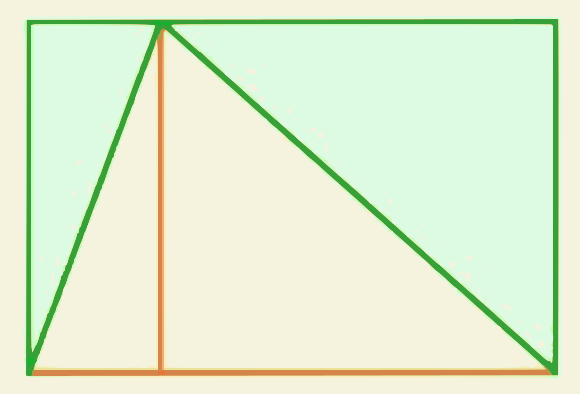
\includegraphics[width=0.6\linewidth]{figures/triangle.png}
%     \caption{We are interested in the area of the orange triangle, which has been split into two.}
%     \label{triangle}
% \end{figure}
% Similarly, we have the celebrated Pythagorean theorem, another formula we have been told to believe. Let $a$ and $b$ be two legs of a right triangle, and $c$ the hypotenuse. We know that $a^2 +b^2 = c^2$. How can we prove this? Take a look at Figure \ref{pyt}, and compute the area of 4 of these right triangles, both individually and by constructing a large square and subtracting the area of the square in the middle.
% \begin{figure}
%     \centering
%     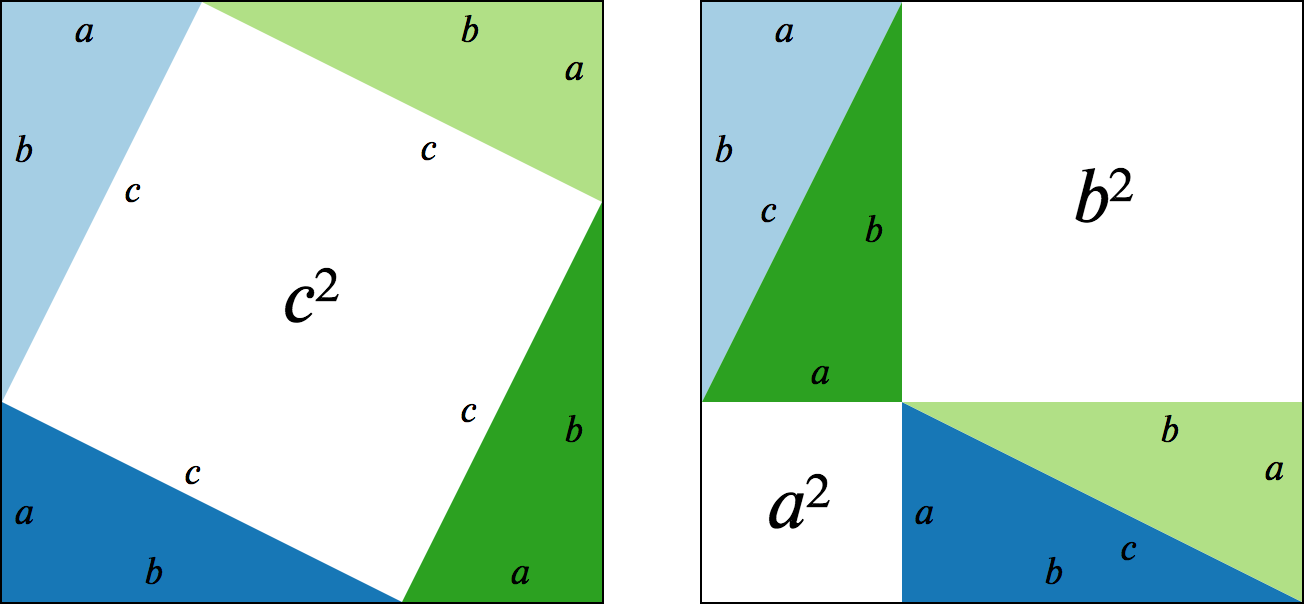
\includegraphics[width=0.6\linewidth]{figures/pythagorean.png}
%     \caption{Compute the area of the colored region both ways to prove the theorem.}
%     \label{pyt}
% \end{figure}
% \begin{align*}
%     4 \frac{1}{2} ab &= (a + b)^2 - c^2\\
%     2ab &= a^2 + 2ab + b^2 - c^2\\
%     c^2 &= a^2 + b^2
% \end{align*}

% Let's get back to the area of a circle. One of the most commonly known proofs is from about two thousand years ago by Archimedes (260 B.C.E.). For an $n$ side regular polygon , its area is going to be $A_n = \frac{1}{2} p_n a_n$, where $p_n$ is the perimeter and $a_n$ is the apothem (distance from center to midpoint of one of the sides). See \href{https://en.wikipedia.org/wiki/Area_of_a_circle#Archimedes's_proof}{Wikipedia} for the full proof. As in Figure \ref{circle}, the inscribed polygon will have perimeter approaching $2\pi R$, and apothem approaching $R$, as $n \rightarrow \infty$. The inscribed polygon also has less area than the circle. Letting $A$ be the area of the circle, we have
% \begin{align*}
%     A \geq \frac{1}{2} p_n a_n
% \end{align*}
% Taking the limit of both sides as $n$ gets large, we have
% \begin{align*}
%     A \geq \frac{1}{2} 2 \pi R \cdot R = \pi R^2
% \end{align*}
% For the circumscribed polygon, the apothem is always $R$, and the perimeter also approaches $2\pi R$. Thus,
% \begin{align*}
%     A \leq \frac{1}{2} p_n a_n = \frac{1}{2} p_n R
% \end{align*}
% Taking the limit once again, we have
% \begin{align*}
%     A \leq \frac{1}{2} 2 \pi &R \cdot R = \pi R^2\\
%     \implies \pi R^2 &\leq A \leq \pi R^2
% \end{align*}
% proving the area formula.

% \begin{figure}
%     \centering
%     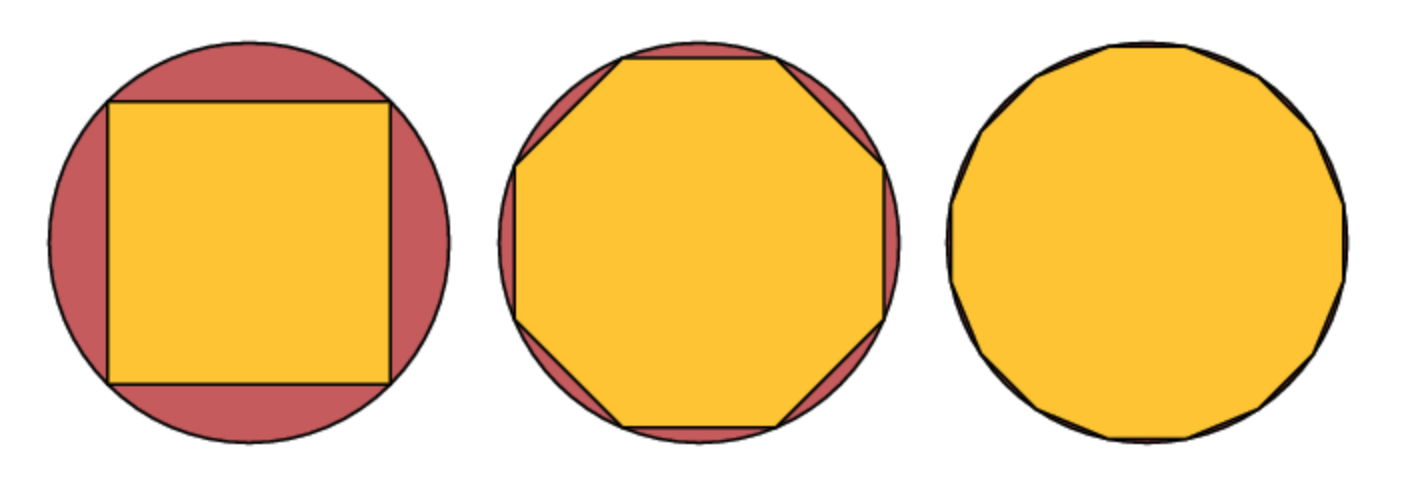
\includegraphics[width=0.6\linewidth]{figures/inscribed.png}
%     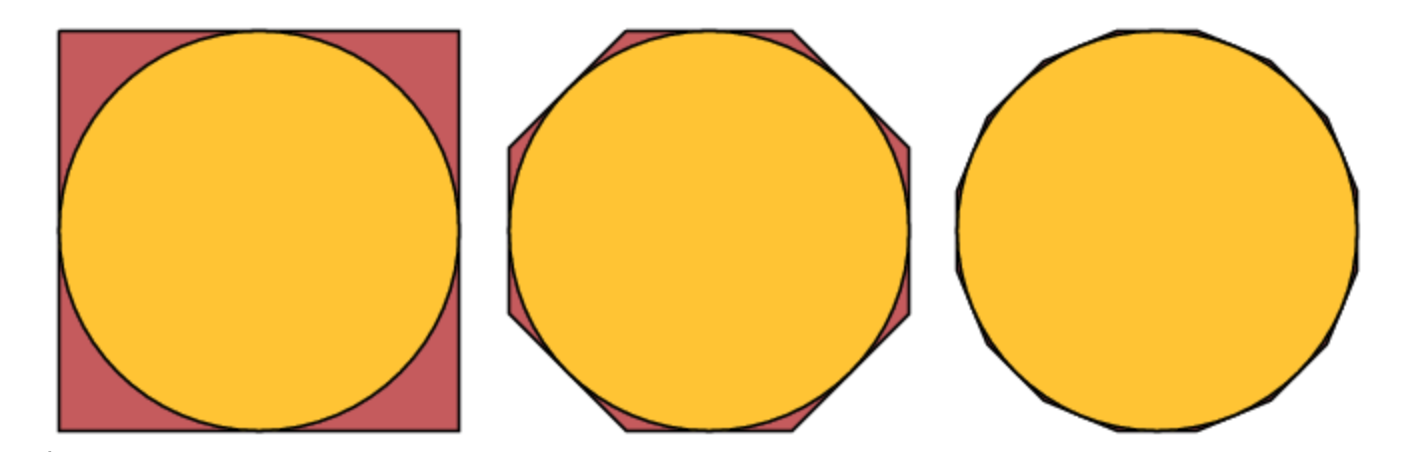
\includegraphics[width=0.6\linewidth]{figures/circumscribed.png}
%     \caption{The first panel shows an inscribed polygon, while the second shows the circumscribed polygon. Both approach the circle in area.}
%     \label{circle}
% \end{figure}


{\it Informal picture ``proofs" of area of triangle, Pythagorean theorem, area of a circle, volume of a sphere, and surface area of a sphere.}\\

Ed Scheinerman, currently the dean of our engineering school, can set the stage for you much better than I can. I especially like the first ten pages. Assuming that you've read through the chapter, you have come across definitions, theorems, and some basic proofs. We will not define ``definition" but take it as an introduction or a name of a mathematical object. In future classes, these should always be memorized and be able to be retrieved from your brain upon request. In order to understand, you must first memorize a little bit. On the other hand, theorems are declaritive statements which can be written of the form ``If [assumptions], then [conclusion]". More on this later.

\begin{defi}[Set]
    A set is a collection of unordered, distinct objects. 
\end{defi}
Sets can have a finite or infinite number of elements, and are usually denoted by capital letters. We can list their elements out one-by-one and wrap then in curly braces, or specify them by some condition, as in $\{x : \text{ condition regarding $x$ is true.}\}$. For example, 
\begin{align*}
    A = \{1, 2, 3, 6, 7\}
\end{align*}
is a set of 5 elements. Letting $\Z = \{..., -1, 0, 1, ...\}$ be the set of all integers, I can denote the same set by
\begin{align*}
    A = \{x \in \Z: 0 < x < 4 \text{ and } 5 < x < 8\}
\end{align*}
The colon within the braces can be read as ``such that". Let $\N = \{0, 1, 2, ...\} = \{x \in \Z: x \geq 0\}$ be the set of natural numbers, or nonnegative integers. Let's recall some definitions from the chapter.
\begin{defi}[Divisible]
    An integer $b$ is divides integer $a$ (written $b \mid a$) if there is an integer $c$ such that $a = bc$. $a$ is called a multiple of $b$, and is also called divisible by $b$. $b$ is also called a divisor or factor of $a$. 
\end{defi}
\begin{defi}[Even]
    An integer $a$ is called even if it is divisible by 2.
\end{defi}
\begin{defi}[Odd]
    An integer $a$ is called odd if there is an integer $x$ such that $a = 2x + 1$.
\end{defi}
\begin{defi}[Prime]
    An integer $p$ is called prime if $p > 1$ and the only positive divisors of $p$ are 1 and $p$.
\end{defi}
\begin{defi}[Composite]
    An integer $c$ is called composite if $c > 1$ and $c$ is not prime. We can also say integer $c > 1$ is composite if there exists a factor $b$ such that $1 < b < c$.
\end{defi}

While none of these concepts are particularly interesting in their own right, they are probably familiar to you. More importantly, with just these definitions, we have a huge class of problems with which to jump in and warm up. 

\begin{exc}
    Prove that the sum of two even integers is even.
\end{exc}
\begin{exc}
    Prove that integer $x$ is even if, and only if, $x + 1$ is odd.
\end{exc}
\begin{exc}
    Prove that the product of an odd and even integer is even.
\end{exc}
\begin{exc}
    Prove that square of an odd integer is odd.
\end{exc}
\begin{exc}
    Prove that square of a prime number is composite.
\end{exc}
\begin{exc}
    Prove that the sum of three consecutive integers is divisible by 3.
\end{exc}
\begin{exc}
    Let $a,b, c$ be integers. Prove that if $a \mid b$ and $b \mid c$, then $a \mid c$.
\end{exc}
\begin{exc}
    Prove that if $n$ is odd, then $-n$ is odd.
\end{exc}
\begin{exc}
    Let $a,b, c$ be integers. Prove that if $a \mid b$ and $a \mid c$, then $a \mid (b+c)$.
\end{exc}
\begin{exc}
    Let $a,b, c$ be integers. Prove that if $a \mid b$ and $a \mid c$, then $a \mid (bc)$.
\end{exc}
\begin{exc}
    Prove that the difference between consecutive perfect squares is odd.
\end{exc}

\begin{exm}
    Let $x$ be an integer. If $x > 1$, then $x^3 + 1$ is composite.
\end{exm}
\begin{proof}
    See page 19 of Scheinerman.
\end{proof}

\begin{exc}
    Provide two conditions $A$ and $B$ such that
    \begin{itemize}
        \item If $A$, then $B$ is true.
        \item If $B$, then $A$ is false.
    \end{itemize}
\end{exc}
\begin{exc}
    Say that you are asked to prove "If $A$ or $B$, then $C$". Why must you show BOTH $A \implies C$ and $B \implies C$? Why not just one?
\end{exc}
\begin{exc}
    Give a counterexample of the ``SSA" postulate for triangle congruence.
\end{exc}
\begin{exc}
    A perfect number is an integer whose divisors add up to the number. For example, $28 = 1 + 2 + 4 + 7 + 14$. Find a perfect number less than 28. Is it the only one? {\it Hint: Try adding additional constraints, such as the number having only two prime factors. Is this a good assumption to make?}
\end{exc}
\begin{exc}
    Disprove: Let $a, b$ be integers. $a \mid b$ and $b \mid a \implies a = b$.
\end{exc}
\begin{exc}
    Disprove: Let $a, b$ be integers. $a \mid b \implies a \leq b$.
\end{exc}
\begin{exc}
    Disprove: Two right triangles have the same area if and only if the lengths of their hypotenuses are the same.
\end{exc}
\begin{exc}
    Disprove: A positive integer is composite if and only if it has two different prime factors.
\end{exc}

\section{January 7, 2020}

\section{January 8, 2020}

\section{January 9, 2020}

% BIBLIOGRAPHY AND ACKNOWLEDGEMENTS
% \paragraph{Acknowledgement} Thank you to the students that attended my section this semester. Your feedback has been extremely helpful, and I hope to see you all around in the spring! Good luck on the final!

% \newpage

% \vspace{5mm}
% \bibliography{refs}
% %\bibliographystyle{IEEEtran}
% \bibliographystyle{plainnat}

% \newpage

\end{document}

